\documentclass[../thesis.tex]{subfiles}
\begin{document}

\chapter{Experiments}
\label{ch:experiments}
In this section, the frame field generation applied to a cuboid
with some different metrics is discussed.

\paragraph{Constant metric}
\begin{figure}[htb]
    \centering
    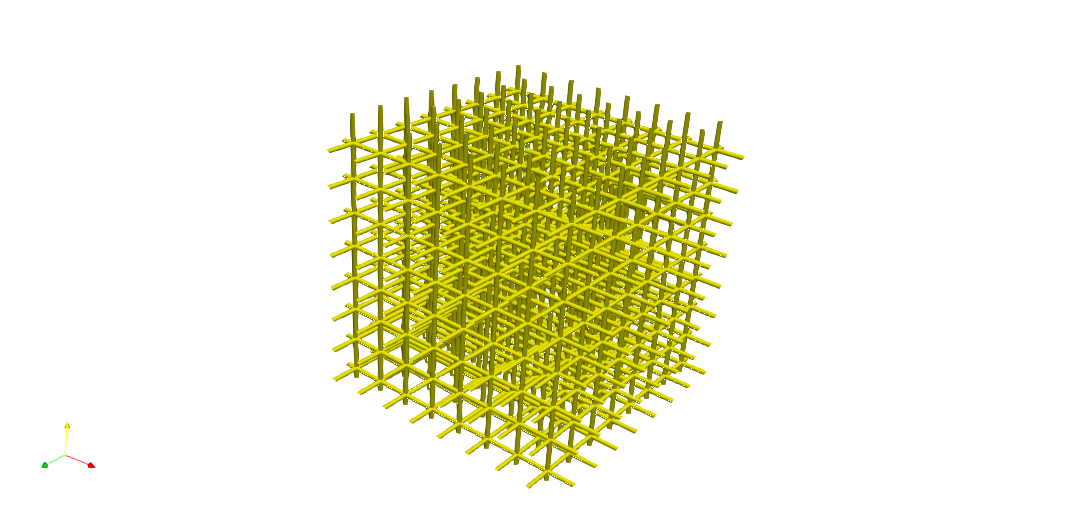
\includegraphics[width=20em]{figures/constant_metric}
    \caption{Idea of quadrangulation with integer-grid maps in 2D}
    \label{fig:constant-metric}
\end{figure}
\begin{itemize}
    \item As a sanity check, we start with the constant metric everywhere.
    
    
    
    constant metric everywhere -> no singularities
    \item linearly increasing metric in z-axis, isotropic scaling
    \item 2d example anisotropic scaling, constant-linear-constant
    \item larger cubes at the edges of the cube, isotropic scaling
\end{itemize}

\end{document}